\documentclass[a4paper]{scrreprt}

% Uncomment to optimize for double-sided printing.
% \KOMAoptions{twoside}

% Set binding correction manually, if known.
% \KOMAoptions{BCOR=2cm}

% Localization options
\usepackage[english]{babel}
\usepackage[T1]{fontenc}
\usepackage[utf8]{inputenc}

% Monospaced font with support for bold
\usepackage[scaled=1.04]{couriers}

% Quotations
\usepackage{dirtytalk}

% Enhanced verbatim sections. We're mainly interested in
% \verbatiminput though.
\usepackage{verbatim}

% Automatically remove leading whitespace in lstlisting
\usepackage{lstautogobble}

% PDF-compatible landscape mode.
% Makes PDF viewers show the page rotated by 90°.
\usepackage{pdflscape}

% Advanced tables
\usepackage{array}
\usepackage{tabularx}
\usepackage{longtable}

% Fancy tablerules
\usepackage{booktabs}

% Graphics
\usepackage{graphicx}

% Current time
\usepackage[useregional=numeric]{datetime2}

% Float barriers.
% Automatically add a FloatBarrier to each \section
\usepackage[section]{placeins}

% Custom header and footer
\usepackage{fancyhdr}

\usepackage{geometry}
\usepackage{layout}

% Math tools
\usepackage{mathtools}
% Math symbols
\usepackage{amsmath,amsfonts,amssymb}
\usepackage{amsthm}

\DeclarePairedDelimiter{\ceil}{\lceil}{\rceil}
\DeclarePairedDelimiter{\floor}{\lfloor}{\rfloor}

% General symbols
\usepackage{stmaryrd}

\DeclarePairedDelimiter\abs{\lvert}{\rvert}

% Indistinguishable operator (three stacked tildes)
\newcommand*{\diffeo}{% 
  \mathrel{\vcenter{\offinterlineskip
  \hbox{$\sim$}\vskip-.35ex\hbox{$\sim$}\vskip-.35ex\hbox{$\sim$}}}}

% Bullet point
\newcommand{\tabitem}{~~\llap{\textbullet}~~}

\pagestyle{plain}
% \fancyhf{}
% \lhead{}
% \lfoot{}
% \rfoot{}
% 
% Source code & highlighting
\usepackage{listings}

% Coloured boxes!
\usepackage[most]{tcolorbox}
\newtcolorbox{library}[2][]{
	enhanced,
	sharp corners,
	coltitle=black, % title colour
	colbacktitle=black!10!white, % title bg colour
	halign title=center, % title align
	toptitle=1mm, % Top/bottom additional spacing for title
	bottomtitle=1mm,
	fonttitle=\ttfamily,
	colback=white, % body bg colour
	fontupper=\ttfamily,
	title=#2,#1
}

\newtcolorbox{boxcomment}[2][]{
	enhanced,
	colframe=white, % frame colour
	colbacktitle=white, % title bg colour
	halign=center, % body align
	colback=white, % body bg colour
	fonttitle=\ttfamily,
	fontupper=\ttfamily,
	title=#2,#1
}

% SI units
\usepackage[binary-units=true]{siunitx}
\DeclareSIUnit\cycles{cycles}

% Convenience commands
\newcommand{\mailsubject}{41100 - Distributed algorithms - Series 5}
\newcommand{\maillink}[1]{\href{mailto:#1?subject=\mailsubject}
                               {#1}}

% Should use this command wherever the print date is mentioned.
\newcommand{\printdate}{\today}

\subject{41102 - Distributed algorithms}
\title{Series 5}

\author{Michael Senn \maillink{michael.senn@students.unibe.ch} - 16-126-880}

\date{\printdate}

% Needs to be the last command in the preamble, for one reason or
% another. 
\usepackage{hyperref}


\begin{document}
\maketitle


\setcounter{chapter}{4}

\chapter{Series 5}

\section{Regular register executions}

\subsection{Read-one write-all}

The first non-concurrent read operation returning $x$ is a direct result of the
validity property of a regular register. When the write operation starts, $p$
will broadcast write messages to all other processes, and will only complete
the write operation once all healthy processes have acknowledge the write. Any
subsequent read by $q$ will then return its local value, which is guaranteed to
be equal to $x$.

For the case of the two concurrent read operations, consider the message
flow in figure \ref{fig:read_one_write_all}. Assume that $p.write(x)$ as
described above took place earlier.

\begin{figure}[h]
    \centering
    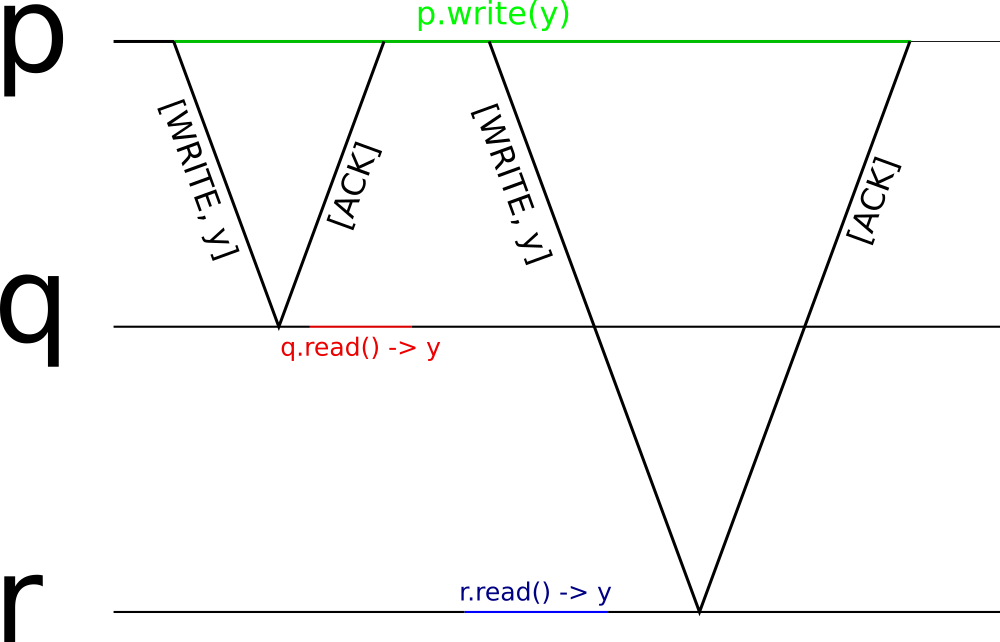
\includegraphics[width=0.7\textwidth]{res/5_1_a.png}
    \caption{Message flow of Read-one write-all algorithm}
    \label{fig:read_one_write_all}
\end{figure}

The local write of $p$ is assumed to happen immediately after the write
operation starts, and as such left out for brevity. A read on $q$ concurrent to
the write on $p$, which happens at a time as shown will return $y$, while a
subsequent read on $r$ will return $x$, as the write message has not arrived at
$r$ yet, leading to the requested execution.


\subsection{Majority voting regular register}

As above, the first non-concurrent read operation returning $x$ follows from
the validity property of the algorithm. The write operation will not finish
before a majority of processes have acknowledged the write. A subsequent
non-concurrent read will then read data from the majority of processes,
guaranteeing that at least one of the read $(wts, v)$ tuples is one of the most
recent write. As the value of the most recent timestamp is then returned, it
will be $x$.

For the case of two concurrent read operations, consider the message flow in
figure \ref{fig:majority_voting}. Assume that $p.write(x)$ as described above
took place earlier.

\begin{figure}[h]
    \centering
    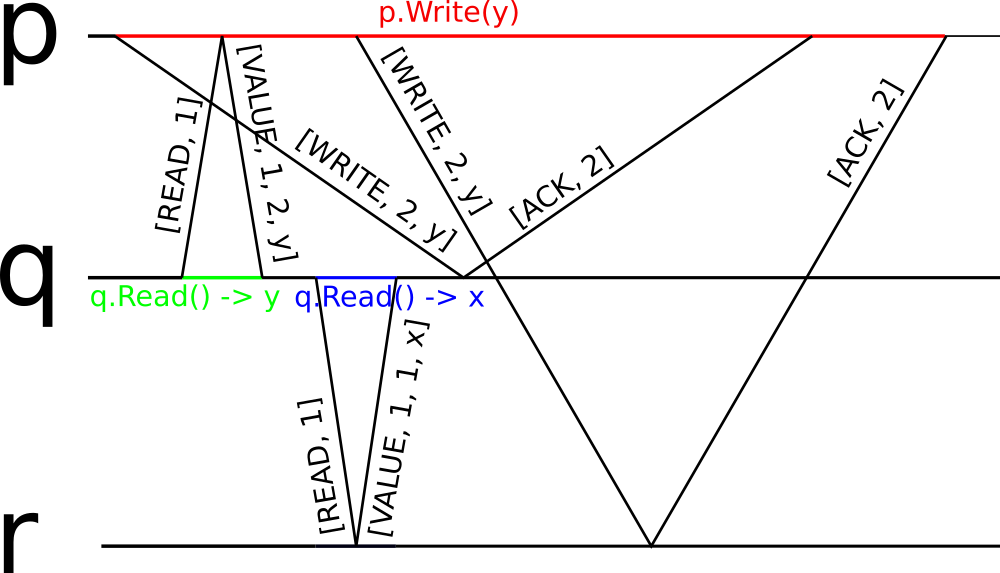
\includegraphics[width=0.9\textwidth]{res/5_1_b.png}
    \caption{Message flow of majority voting algorithm}
    \label{fig:majority_voting}
\end{figure}

Local write and read operations are assumed to happen immediately, with
messages left out for brevity.

A read on $q$ concurrent to a write on $p$ might read the values stored within
$q$ and $p$, with no read from $r$ due to eg delays in communication. Such a
read satisfies the majority criteria and will, as $p$ contains the value and
timestamp of the concurrent write operation, return $y$.

A subsequent read on $r$ might read the local data as well as data from $q$
which once again satisfies the majority criteria. As it might do so before the
write messages from $p$ have arrived at eitehr $q$ or $r$, the returned value
will hence be $x$.

\section{Read-all write-one regular register}

\begin{library}{Implementing read-all write-one regular register}
  \begin{lstlisting}[mathescape=true,autogobble=true,breaklines=true,escapeinside={<@}{@>},basicstyle=\small]
    <@\textbf{Implements}@>:
      $(1, N)$ regular register, <@\textbf{instance}@> onrr

    <@\textbf{Uses}@>:
      BestEffortBroadcast, <@\textbf{Instance}@> $beb$
      PerfectPointToPointLinks, <@\textbf{Instance}@> $pl$
      PerfectFailureDetector, <@\textbf{Instance}@> $P$

    <@\textbf{upon event}@> $(onrr, Init)$ <@\textbf{do}@>:
      $val := \bot$
      $correct := \Pi$
      $readset := \emptyset$
      $valueset := \emptyset$
      $wid := 0$

    <@\textbf{upon event}@> $(P,\ Crash\ |\ p)$ <@\textbf{do}@>:
      $correct := correct \setminus \{p\}$

    <@\textbf{upon event}@> $(onrr,\ Write\ |\ v)$ <@\textbf{do}@>:
      $wid := wid + 1$
      $val := v$
      <@\textbf{trigger}@> $(onrr,\ WriteReturn)$

    <@\textbf{upon event}@> $(onrr,\ Read)$ <@\textbf{do}@>:
      <@\textbf{trigger}@> $(beb,\ Broadcast\ |\ [READVALUE])$

    <@\textbf{upon event}@> $(beb,\ Deliver\ |\ q,\ [READVALUE])$ <@\textbf{do}@>:
      <@\textbf{trigger}@> $(pl,\ Send\ |\ q,\ [VALUE,\ val,\ wid])$

    <@\textbf{upon event}@> $(pl,\ Deliver\ |\ q,\ [VALUE,\ val,\ wid])$ <@\textbf{do}@>:
      $readset := readset \cup \{q\}$
      $valueset:= valueset \cup \{(val,\ wid)\}$

    <@\textbf{upon event}@> $(correct \subseteq readset)$ <@\textbf{do}@>:
      // As only one writer, also the only tuple with wid != 0
      out := $v \text{ for } (v,\ wid) \in valueset \text{ with largest } wid$

      $readset := \emptyset$
      $valueset := \emptyset$

      <@\textbf{trigger}@> $(onrr,\ ReadReturn\ |\ out)$

  \end{lstlisting}
\end{library}

\section{$(1, 1)$ atomic register}

\end{document}
